
\documentclass[12pt,english]{article}

\usepackage[latin9]{inputenc}
\usepackage{geometry}
%\usepsackage{babel}
\usepackage{amsthm}
\usepackage{amsmath}
\usepackage{amssymb}
\usepackage{graphicx}
\usepackage{setspace}
\usepackage{hyperref}
 \usepackage{cleveref}
 \usepackage{topcapt, lscape}
 \usepackage{rotating}
 \usepackage{booktabs}
 \usepackage[para]{threeparttable}
%\usepackage{breakurl}
\usepackage{color}
\usepackage{harvard}
\usepackage{float}
\usepackage{topcapt, lscape}
%\setcounter{MaxMatrixCols}{10}
\usepackage{scalefnt}
%\usepackage{ulem}
\newcommand{\note}[1]{\footnote{ \begin{doublespace}#1  \end{doublespace}}}

\usepackage[para]{threeparttable}
\geometry{verbose,tmargin=1.25in,bmargin=1.25in,lmargin=1in,rmargin=1in}
\setlength{\parskip}{0.1in}
\setlength{\parindent}{0pt}
\makeatletter
\newcommand{\lyxdot}{.}
\numberwithin{equation}{section}


\theoremstyle{plain}
\newtheorem{thm}{\protect\theoremname}

\newtheorem{assumption}{\protect\assumptionname}
\theoremstyle{remark}

\newtheorem*{rem*}{\protect\remarkname}
\newtheorem{rem}{\protect\remarkname}[section]
  \theoremstyle{plain}

\newtheorem{lem}{\protect\lemmaname}
  \providecommand{\assumptionname}{Assumption}
  \providecommand{\lemmaname}{Lemma}
  \providecommand{\remarkname}{Remark}
\providecommand{\theoremname}{Theorem}
\makeatother
  \providecommand{\assumptionname}{Assumption}
  \providecommand{\lemmaname}{Lemma}
  \providecommand{\remarkname}{Remark}
\providecommand{\theoremname}{Theorem}
\newcommand{\red}[1]{\textcolor{red}{#1}}
\newcommand{\blue}[1]{\textcolor{blue}{#1}}


\begin{document}

\subsection{Estimating CFscores in Brazil}

\bigskip \Large 
\red{revisar desde aca}
\bigskip \normalsize

\red{include in this section all the robustness checks (some are before)}

\subsection{from before}

The intuition for how campaign contributions can be used to estimate politicians' policy positions is similar in spirit to that behind DW-Nominate. % In the latter, $K$ legislators face a sequence of decisions between two alternatives, which are unobservable for the econometrician. If legislators' ideal points were known, we can think of the estimation problem as finding separating hyperplanes (or midpoints in one dimension) that minimize incorrect classification of predicted yay and nay votes. If instead all separating hyperplanes were known, ideal points for each legislator are again found by minimizing classification errors across roll calls. We can think of an algorithm behind DW-Nominate as alternating between one and the other step, until convergence. With campaign contribution data, each contributor takes the role of a roll call, and their contributions of the separating hyperplanes (extended, of course, from a binary choice to a continuum). 
 The key assumption is that the contributor's marginal benefit of giving to a particular candidate is decreasing in the distance between the contributor's ideal policy and the candidate's choice. This implies that contributors give (weakly) more money to candidates that are closer to their ideal point, which in turn allows us to rank candidates' positions in the policy space. Bonica interprets these estimates as politicians' policy preferences. We only make the assumption that these are the candidates' policy positions, which could or not correspond with their true preferences.\footnote{Estimation is carried out by a modified correspondence analysis, where we first construct a two-way frequency matrix, where rows are unique contributors and columns, candidates. Each element in that matrix is the total amount of contributions made by contributor $i$ to candidate $j$, for the time span of our dataset. We then perform a singular value decomposition to retrieve ideal points for contributors and recipients.}  
 
 
\subsection{gali}
The intuition for recovering policy positions from campaign contributions is as follows. Firstly, each contributor allocates their campaign contributions to political candidates who are close to them ideologically. In general, candidates that are closer ideologically should receive similar patterns in contribution with respect to contributors than candidates who are ideologically dissimilar. Ideological proximity between politicians, in this context, is measured with respect to the frequency of donations across rows (contributors), and vice versa for contributors. Intuitively, political candidates who receive similar contribution patterns from the same voters are close together in the factor score.

We estimate CFScores using the methodology outlined in Bonica 2014 and built upon by the Database on Ideology, Money in Politics and Elections.\footnote{Accessed \href{https://web.stanford.edu/~bonica/data.html}{here}.} The first step involves constructing a $n$ by $m$ contingency matrix $R$, where each row $i \in n$ denotes a contributor and each column $j \in k$ denotes a political candidate. Each entry in the contingency matrix corresponds to the sum of contributions across all electoral cycles available for each dyad of contributor to federal and state-level candidates. Note that we exclude corporate donors, as well as political parties who can allocate their resources strategically to politicians. After normalizing the contribution-matrix and extracting residuals, we perform a singular value decomposition (SVD) that allows us to recover CFscore estimates of each political candidate and contributor.\footnote{Note that because most contributors are small-scale, one-off contributors, their CFscore estimates tend to be less reliable than that of politicians who accumulate many contributions.} Anchoring to the left and to the right is accomplished by setting two parties, the PFL and PC do B as right and left respectively.\footnote{This anchoring is motivated by the roll-call ideology estimation by Power and Zucco (2009) which finds these two parties as the right and left-most parties, ideolgically.} Finally, following Bonica 2014, our estimates are normalized to have a mean of 0 and standard deviation of 1.

Note that, in contrast with U.S. elections, Brazilian elections take place in two distinct cycles: federal and state-level elections, as well as municipal elections. These cycles take place in two-year intervals. 


% \begin{figure}[H]
% \begin{center}$
% \begin{array}{cc}
% 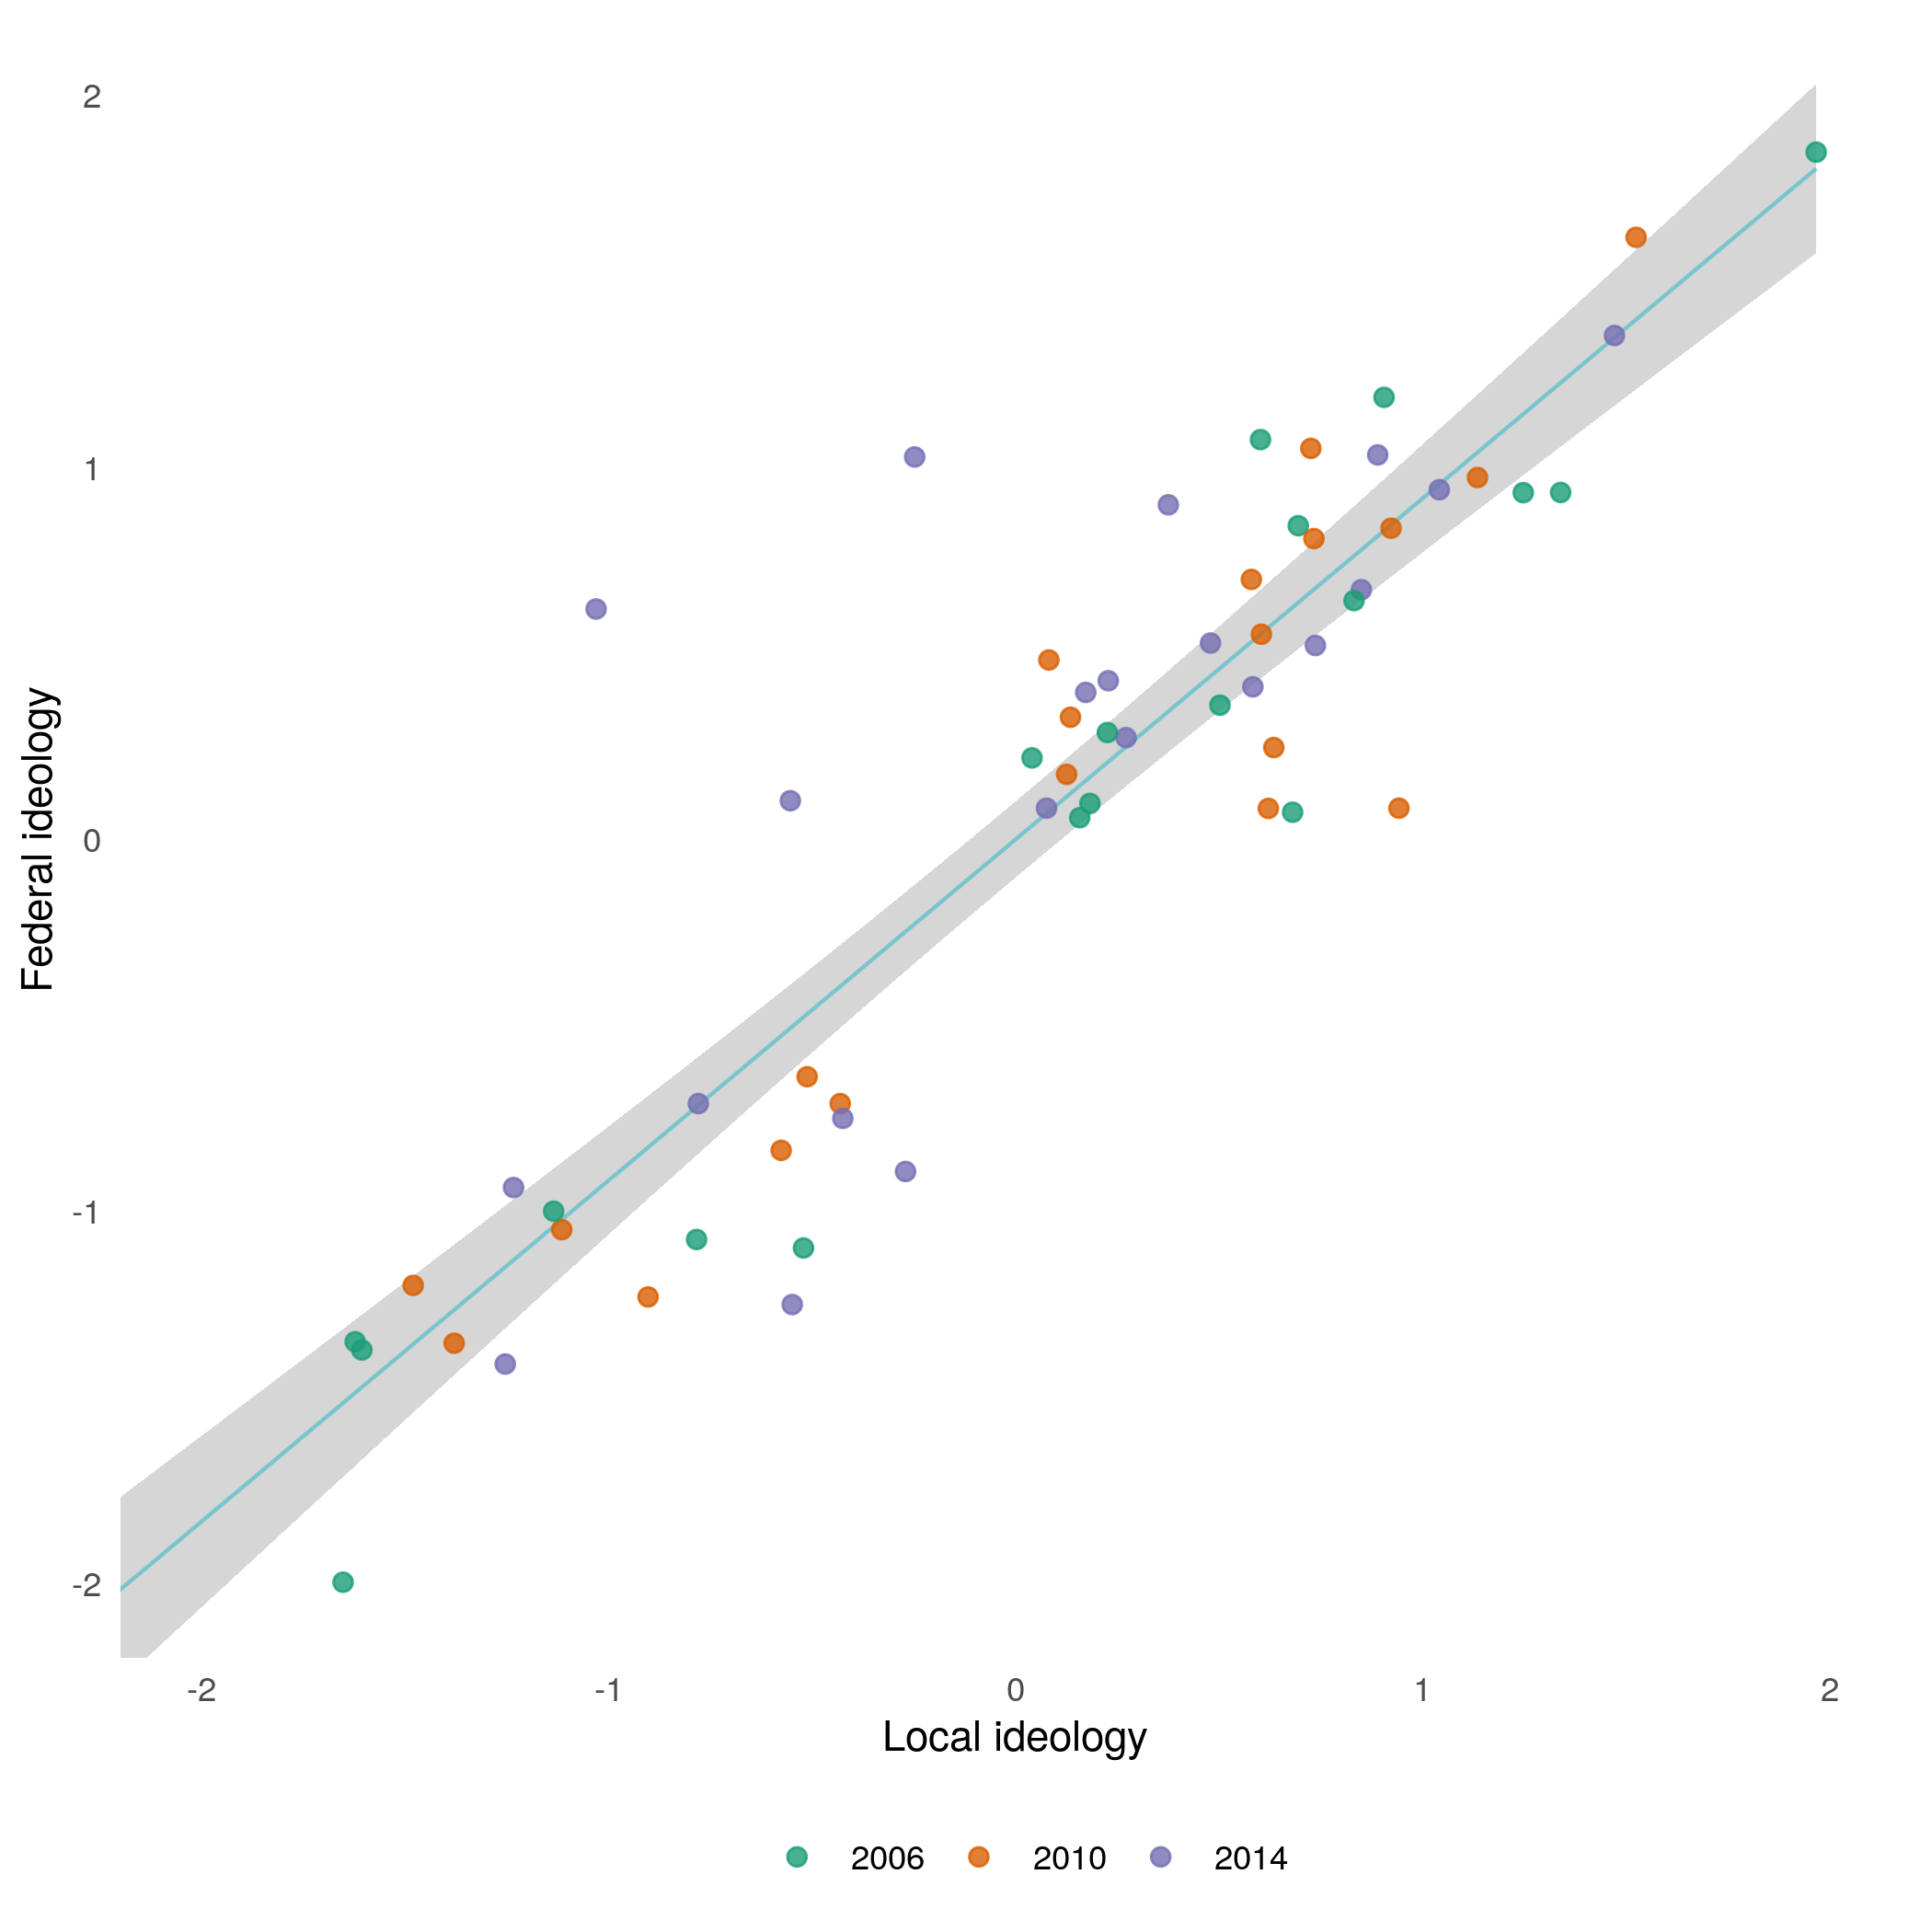
\includegraphics[width=6cm]{\lyxdot /Presentation/figs/ideology/reg_ideology.png} &
% 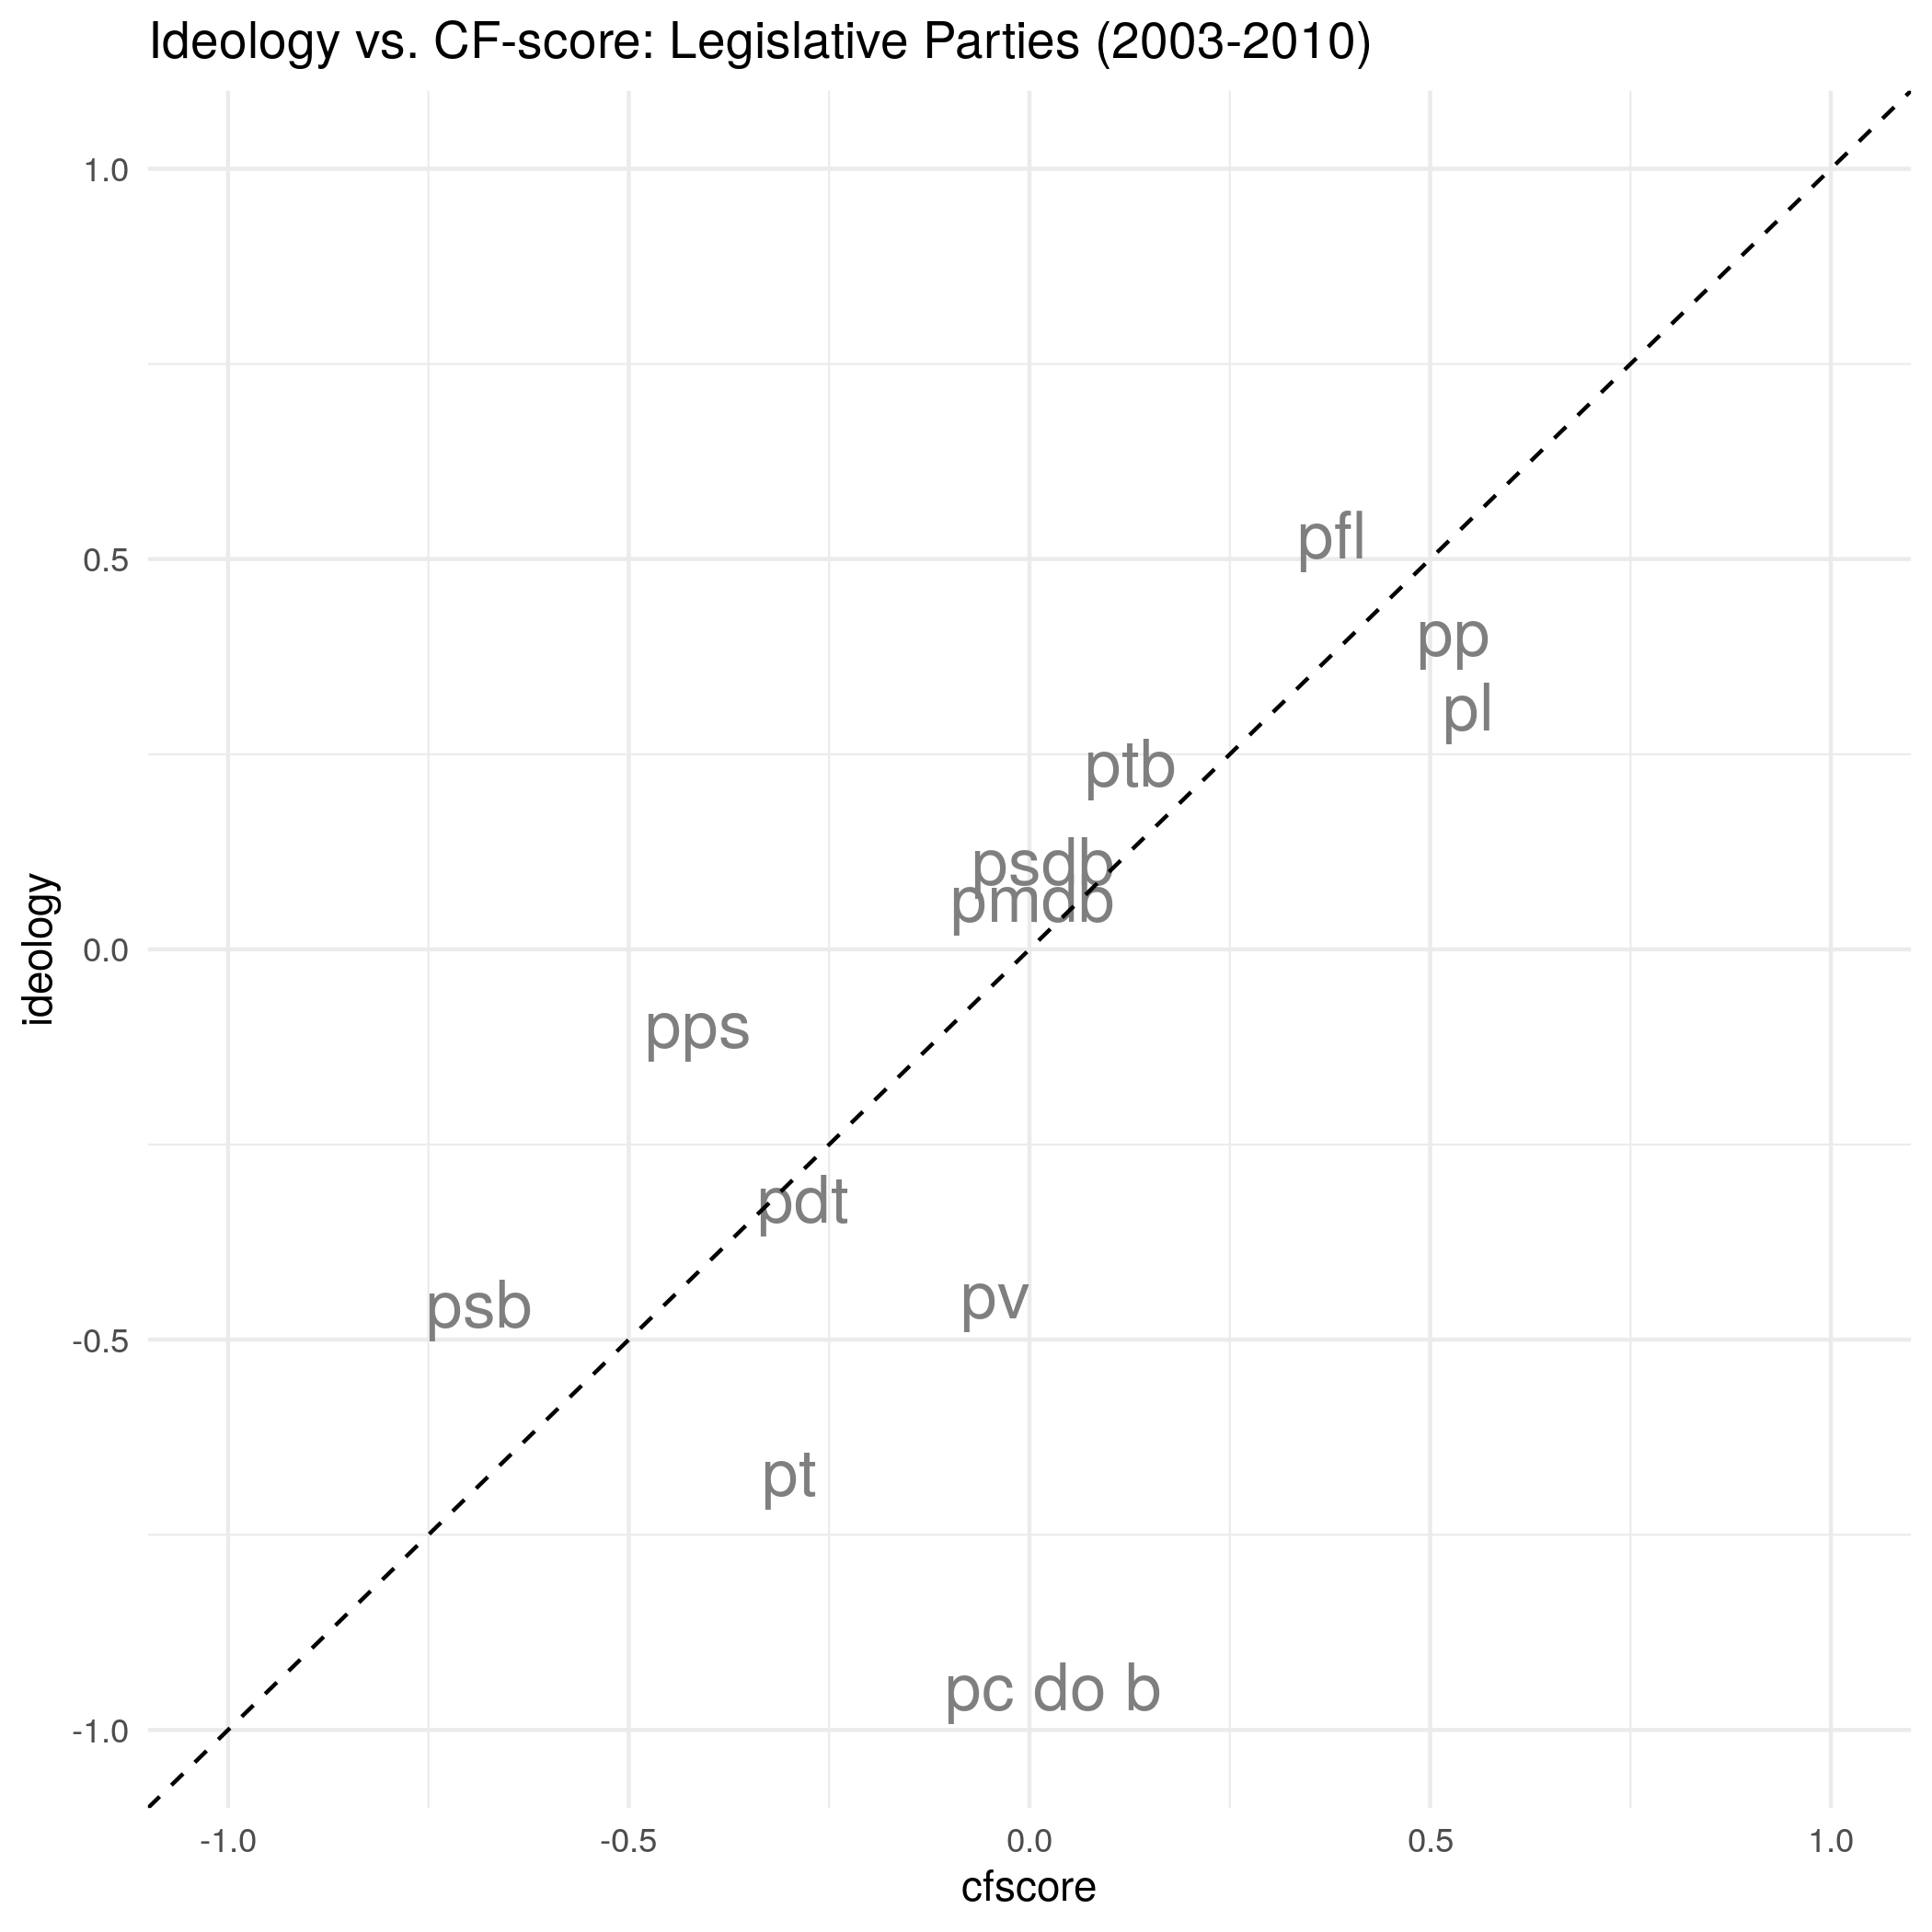
\includegraphics[width=6cm]{\lyxdot /Presentation/figs/ideology/ideology_cfscore.png} 
% \end{array}$
% \end{center}
% \caption{\red{CHECK:  LABELING IS NOT RIGHT. CAPTION IS POOR TOO}Face Validity of Policy Measure.}
%  \label{fig:sanitycheck1}
% \end{figure}



% \begin{figure}[H]
% \begin{center}$
% \begin{array}{cc}
% 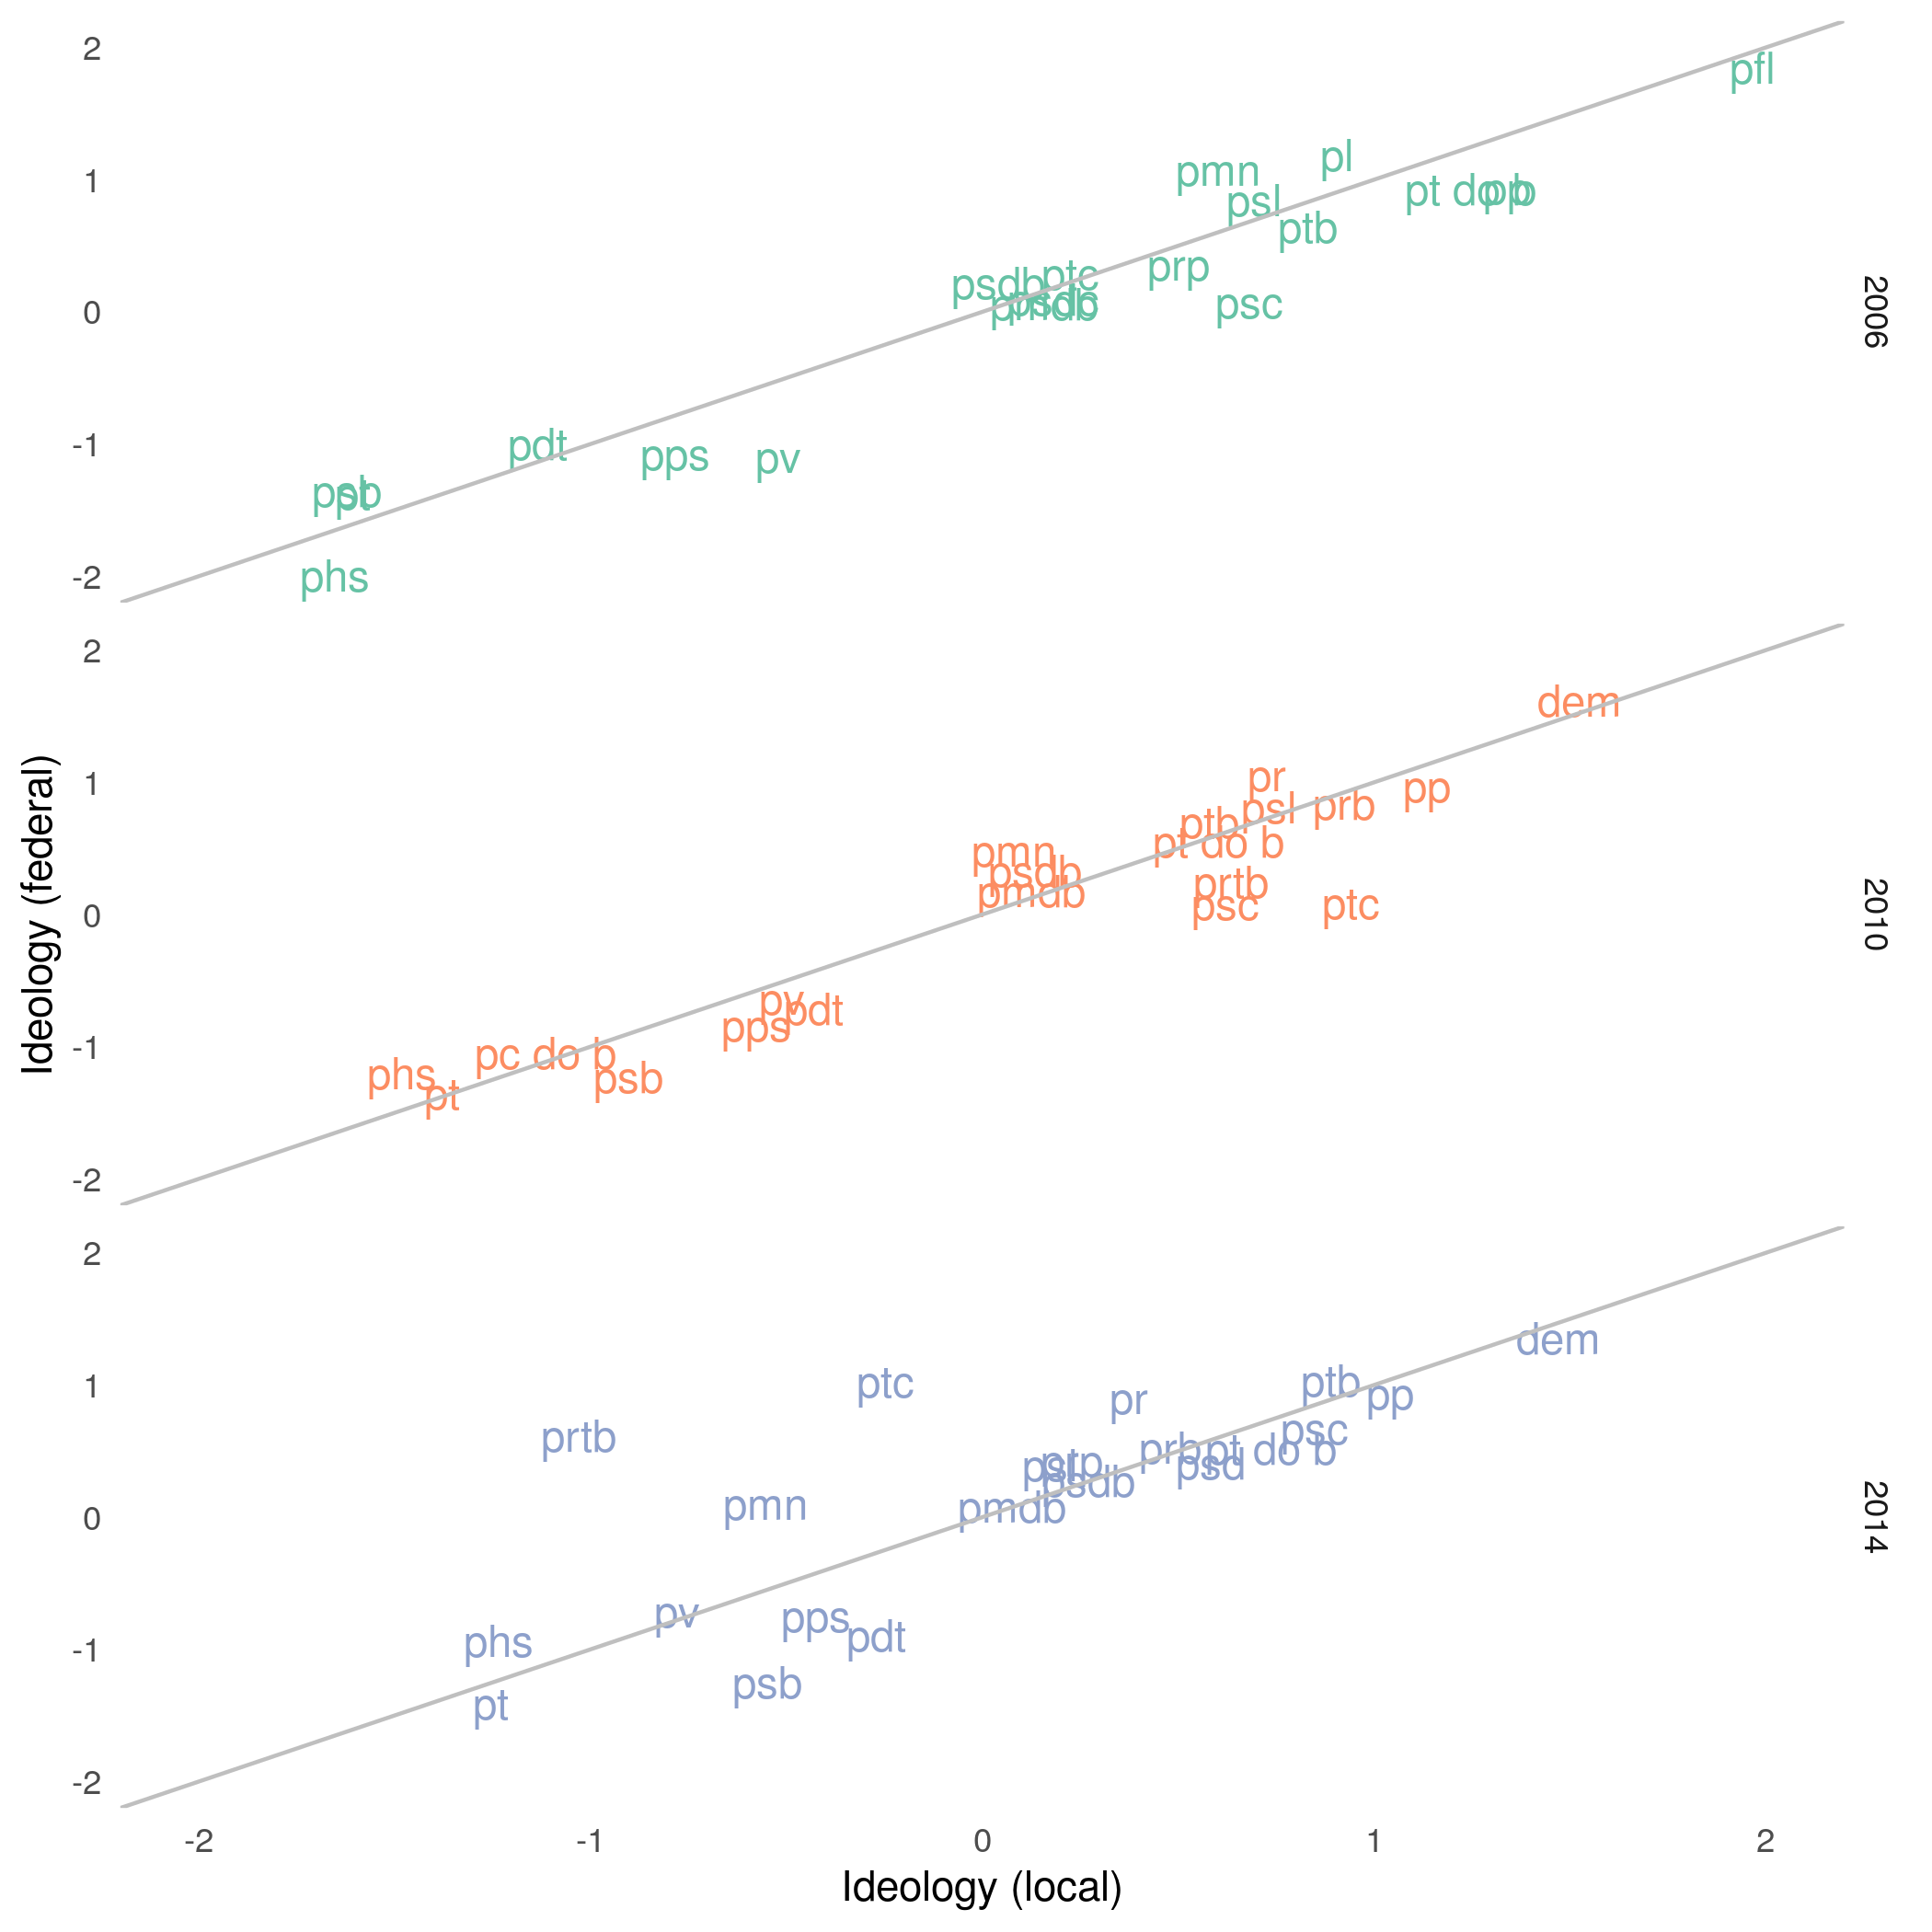
\includegraphics[width=6cm]{\lyxdot /Presentation/figs/ideology/party_ideology_deputy_mayor.png} &
% 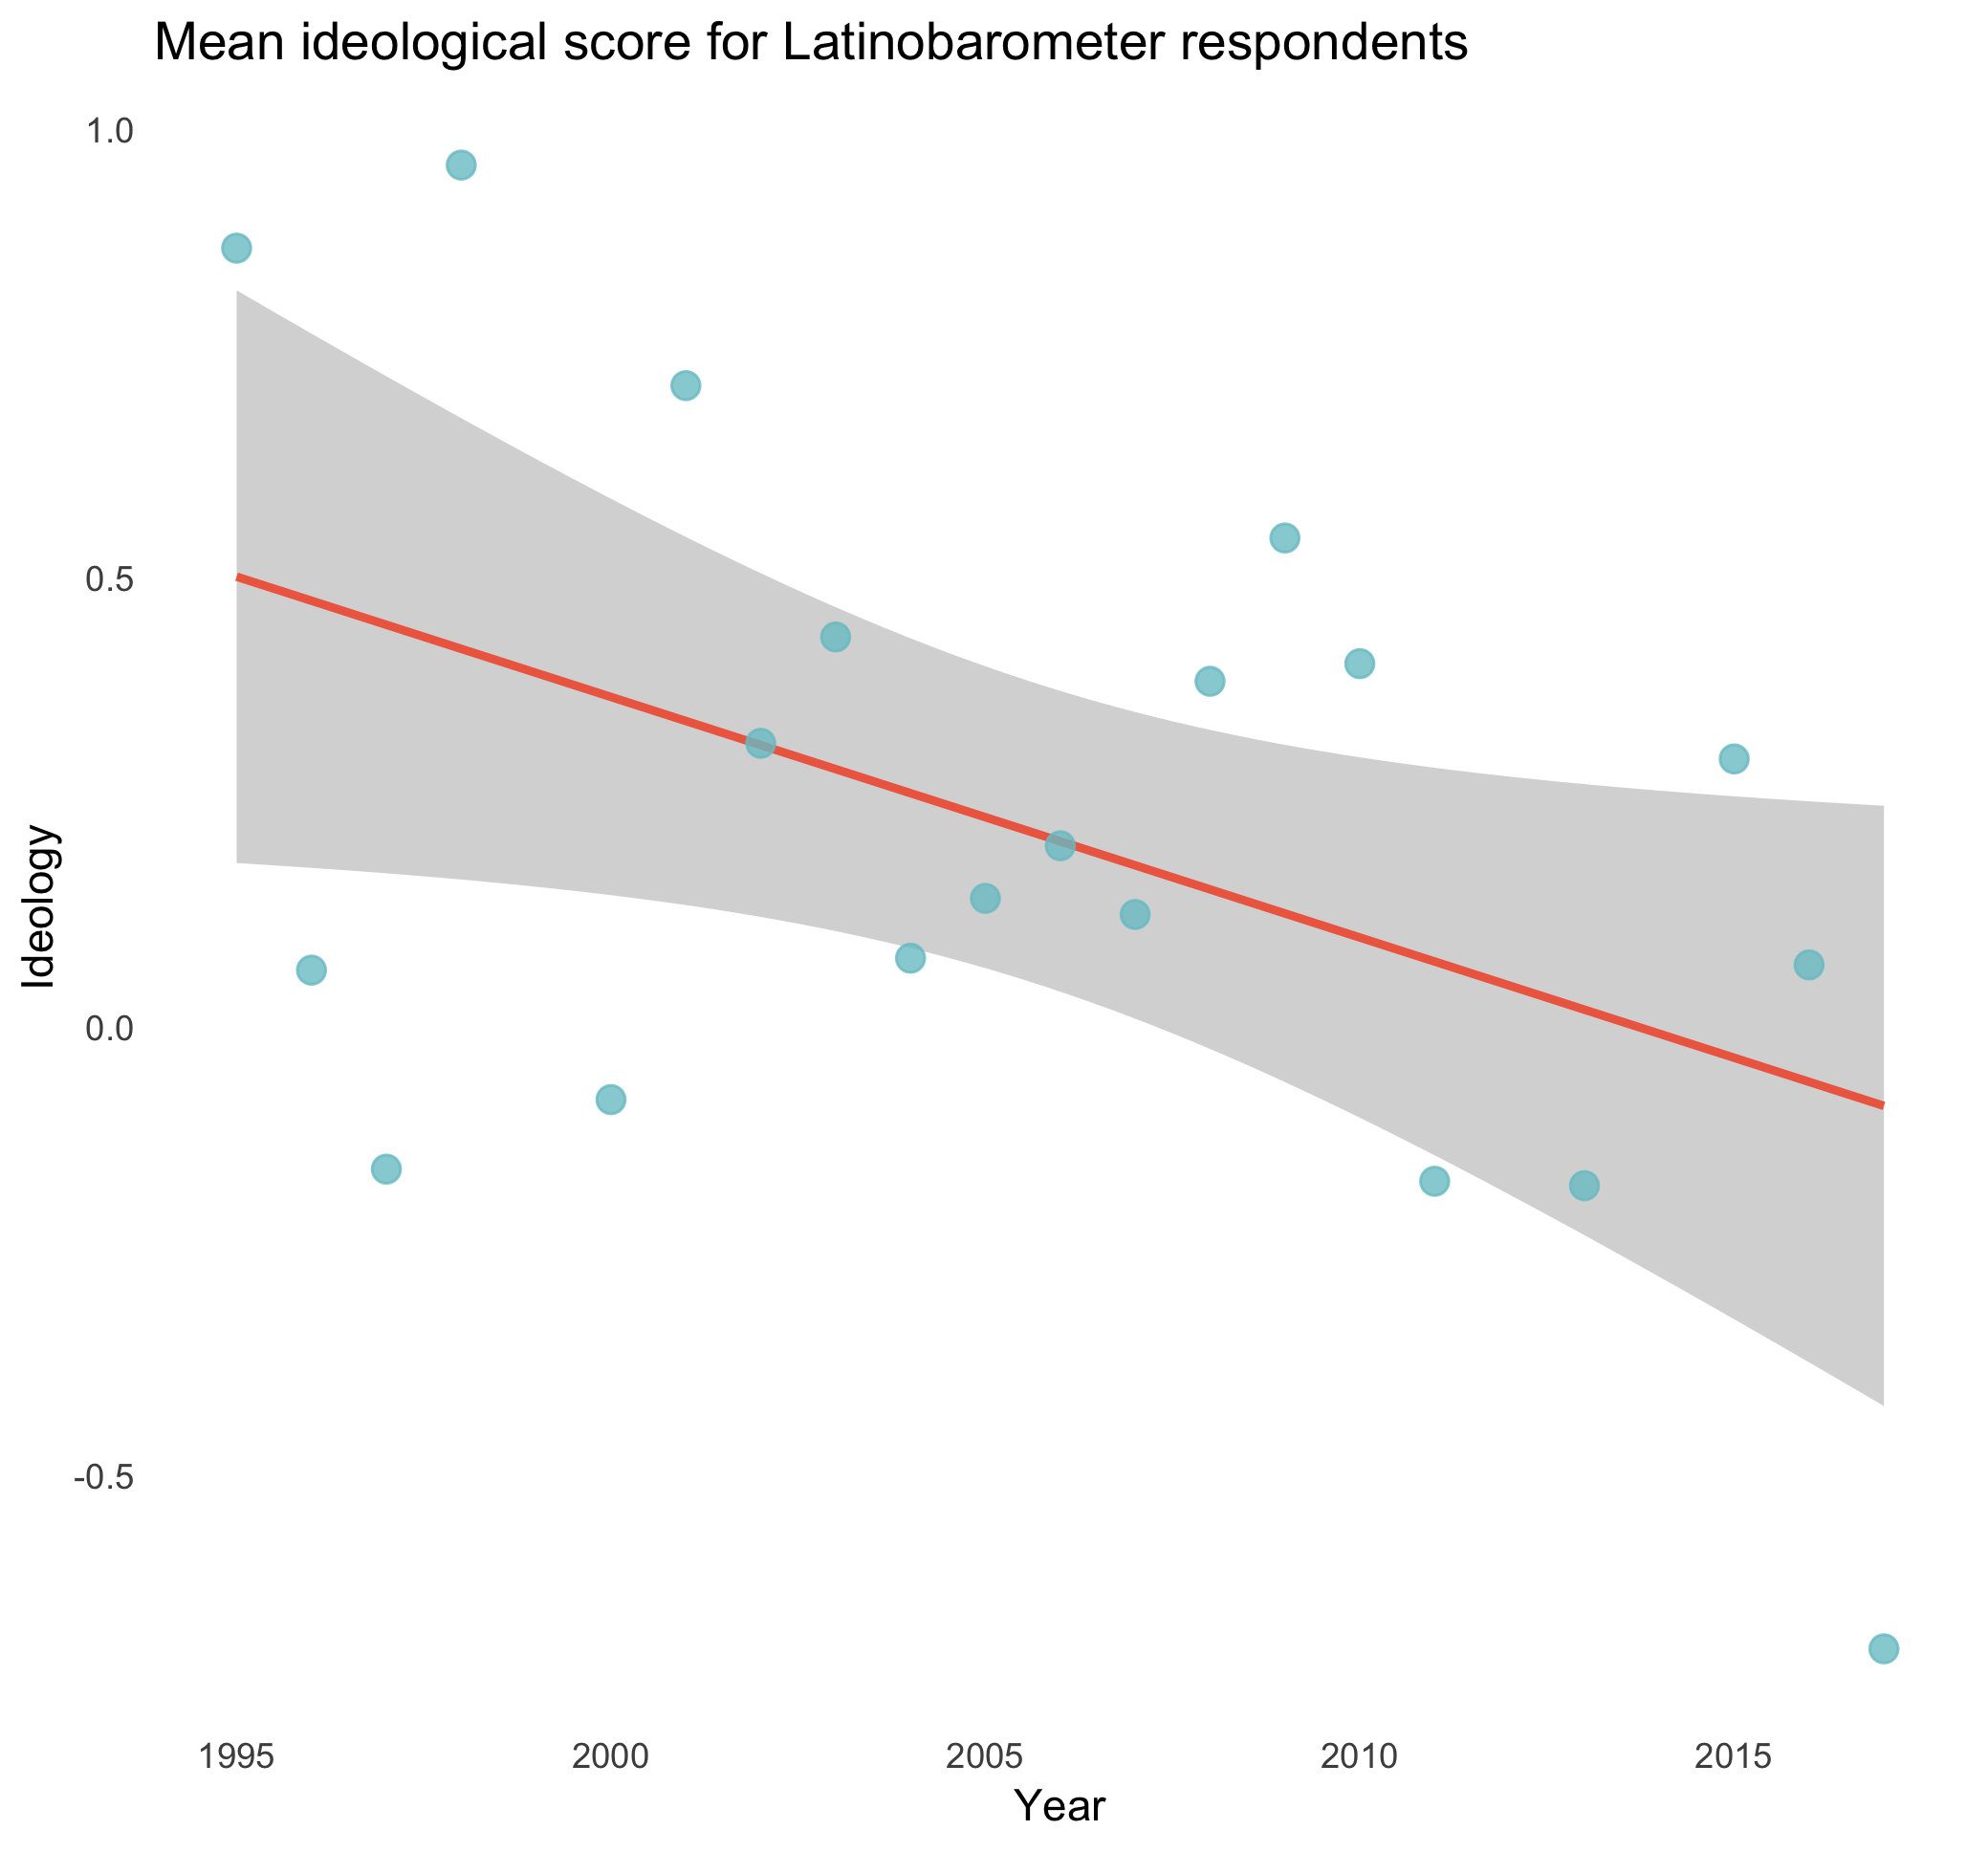
\includegraphics[width=6cm]{\lyxdot /Presentation/figs/ideology/reg_electorate_ideology.png} 
% \end{array}$
% \end{center}
% \caption{\red{CHECK. LABELING IS NOT RIGHT. CAPTION IS POOR TOO}Progressive Movement to the Left of the Ideological Spectrum: in our estimates (left) and in Latinborometer surveys (right). }
%  \label{fig:sanitycheck2}
% \end{figure}

There are well-established concerns regarding corruption in Brazil, in the wake of the largest corruption scandal in Latin America with Operation Carwash. As a result, it is possible that campaign donors may find it worthwhile to donate to candidates in return for public funds or bribes. To address this possibility, we conduct a set of validation exercises to verify if 1) our estimates for candidate ideology are sensitive to excluding largest individual donors and 2) if individual campaign donations are motivated by the possibility of contract allocation. We find no evidence for either hypothesis.

% \begin{figure}[h]
%     \centering
%     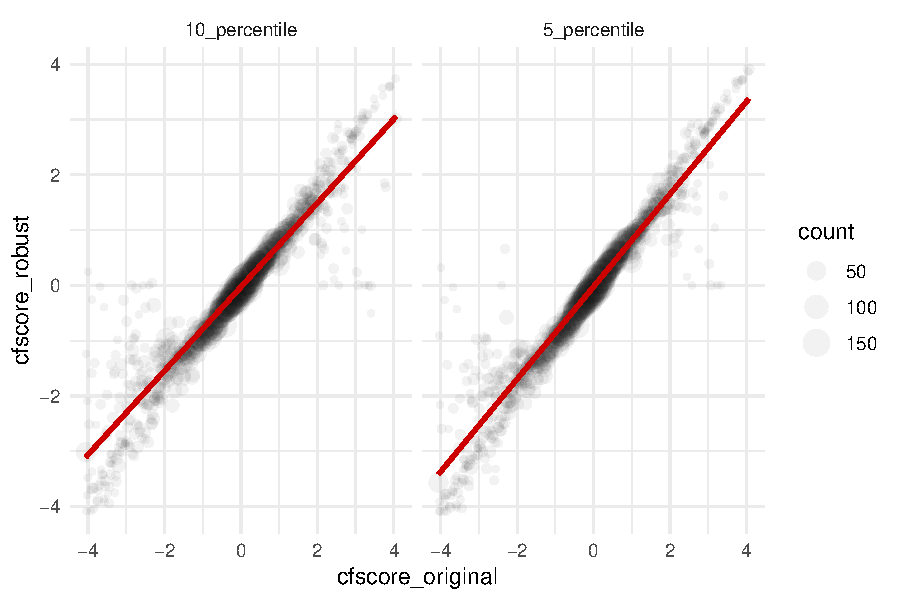
\includegraphics [height=10cm] {./Presentation/figs/ideology/cfscore_robustness.pdf}
%     \caption{\textbf{Policy estimation excluding 5th and 10th percentile.} For each candidate we recompute their policy positions excluding the top 5 and 10 percentile in donors respectively.}
%     \label{fig:cfscore_percentile}
%  \end{figure}

First, we rerun our estimations of candidate policy positions excluding top 5 and 10 percentile donors. Our new estimates have a correlation of 0.9 and 0.847 respectively with the original sample. In figure \ref{fig:cfscore_percentile}, we present a visualization of the new estimates compared to our estimates using the full sample. These findings suggest that our estimates of policy are robust to excluding more generous donors, that may be motivated by other concerns than purely policy preference.

Lastly, to address the concern that campaign donors may be motivated by public contracts, we use the data on public contract allocation by deputado federal provided by Hidalgo, Boas and Richardson (2014). We recover the value of contracts disbursed by elected deputados federais in the mandate of 2006-2010 and assess whether it predicts individual campaign donations by the same candidates in the 2010-2014 cycle. Figure \ref{fig:campaign_contract} shows a scatterplot of total logged contracts by candidate and total individual donations received in 2010. We find that there is no significant relationship between these two, suggesting that individual campaign contributors are not motivated by the potential for contract allocations.

%  \begin{figure}[h]
%      \centering
%      \includegraphics[height=10cm]{./Presentation/figs/ideology/validation_contracts_contribution.pdf}
%      \caption{Estimating the assoiation between total contracts disbusrsed and the amount of individual contributors received in the subsequent electoral cycles. Note that the line is flat, suggesting at most a weak relationship between contract disbursements and donations.}
%      \label{fig:campaign_contract}
%  \end{figure}
 
 

\end{document}